% \documentclass[12pt]{article}
% \usepackage{geometry}
% \geometry{letterpaper}
% \usepackage{graphicx}
% \usepackage{setspace}
% \usepackage{amsmath}
% \usepackage[labelfont=bf,labelsep=period]{caption}
% \renewcommand{\figurename}{Fig.}
% \usepackage{url}
%
% \usepackage[round]{natbib}
% \bibpunct{(}{)}{;}{a}{}{;}
%
% \hyphenation{meta-pop-ulation meta-pop-ulations sub-pop-ulations sub-pop-ulation}
%
% \newcommand{\CV}{\mathrm{CV}}
%
\chapter{Quantifying metapopulation portfolio effects}{Ecological prophets:\\Quantifying metapopulation portfolio effects
} \footnote{A version of this chapter appears as Anderson, S.C., A.B. Cooper, N.K. Dulvy. Ecological prophets: Quantifying metapopulation portfolio
effects. Methods in Ecology and Evolution. 4(10): 971-981.
\url{http://doi.org/10.1111/2041-210X.12093}.}

% \author{Sean C. Anderson$^{1*}$ \and Andrew B. Cooper$^2$ \and Nicholas K. Dulvy$^1$}
%
% \date{}
%
% \textheight 20.5cm
%
% \setcounter{secnumdepth}{-2}
%
% \newcommand{\tilmanPE}{mean-variance PE}
% \newcommand{\schindlerPE}{average-CV PE}
% \newcommand{\zvalue}{$z$-value}
%
% \newcommand{\drivers}{Fig.~\ref{fig:PE-drivers}}
% \newcommand{\driverszcol}{Fig.~\ref{fig:PE-drivers-z-colour}}
% \newcommand{\driverscor}{Fig.~\ref{fig:factors-cor}}
%
%
% \newlabel{fig:didactic}{{1}{25}}
% \newlabel{fig:lines}{{2}{26}}
% \newlabel{fig:meta}{{3}{27}}
% \newlabel{fig:detrend}{{4}{28}}
% \newlabel{fig:paramspace}{{5}{29}}
% \newlabel{fig:recommendations}{{6}{30}}
% \newlabel{tab:datasources}{{S1}{9}}
% \newlabel{tab:ris-meta}{{S2}{10}}
% \newlabel{tab:grb-meta}{{S3}{11}}
% \newlabel{fig:ts}{{S1}{12}}
% \newlabel{fig:map}{{S2}{13}}
% \newlabel{fig:Taylor-fits}{{S3}{14}}
% \newlabel{fig:z-vals}{{S4}{15}}
% \newlabel{fig:inter-vs-intra-z}{{S5}{16}}
% \newlabel{fig:meta-quad}{{S6}{17}}
% \newlabel{fig:meta-lin-quad-avg}{{S7}{18}}
% \newlabel{fig:meta-detrend}{{S8}{19}}
% \newlabel{fig:meta-detrend-loess}{{S9}{20}}
% \newlabel{fig:paramspace-labels}{{S10}{21}}
% \newlabel{fig:PE-predicted-observed}{{S11}{22}}
% \newlabel{fig:factors-cor}{{S12}{23}}
% \newlabel{fig:PE-as-an-index}{{S13}{24}}
%
% \begin{document}
% \begin{spacing}{1.3}

% \maketitle
%
% \noindent
%   \textsuperscript{1}Earth to Ocean Research Group, Department of Biological
%   Sciences, Simon Fraser University, Burnaby BC, V5A 1S6, Canada
%
% \noindent
% 	\textsuperscript{2}School of Resource and Environmental Management, Simon
%   Fraser University, Burnaby, BC, V5A 1S6, Canada
%
% \noindent
% 	\textsuperscript{*}Corresponding author: sean\_anderson@sfu.ca
%
%   \bigskip
% \noindent
% Running title: Quantifying portfolio effects

% \bigskip
% \bigskip
% \noindent
% \texttt{This is the preprint version of the following article:\\
% Anderson, S.C., A.B. Cooper, N.K. Dulvy. Ecological prophets: Quantifying metapopulation portfolio effects. Methods in Ecology and Evolution.\\
% It has been published in final form at:\\
% \url{http://dx.doi.org/10.1111/2041-210X.12093}}
%
% \newpage
\chapter[Quantifying metapopulation portfolio effects]{Ecological
  prophets: Quantifying metapopulation portfolio effects\footnote{A version
    of this chapter appears as Anderson, S.C., A.B. Cooper, N.K. Dulvy.
    Ecological prophets: Quantifying metapopulation portfolio effects. Methods
    in Ecology and Evolution. 4(10): 971-981.
    \url{http://doi.org/10.1111/2041-210X.12093}.}}

\section{Abstract}
\begin{enumerate}
 \item A financial portfolio metaphor is often used to describe how population
   diversity can increase temporal stability of a group of populations. The
   portfolio effect (PE) refers to the stabilizing effect from a population
   acting as a group or ``portfolio'' of diverse subpopulations instead of a
   single homogeneous population or ``asset''. A widely used measure of the PE
   (the average-CV PE) implicitly assumes that the slope (z) of a log-log plot
   of mean temporal abundance and variance (Taylor's power law) equals two.

 \item Existing theory suggests an additional unexplored empirical PE that
   accounts for z, the mean-variance PE. We use a theoretical and empirical
   approach to explore the strength and drivers of the PE for metapopulations
   when we account for Taylor's power law compared to when we do not. Our
   empirical comparison uses data from 51 metapopulations and
   1070 subpopulations across salmon, moths, and reef fishes.

 \item Ignoring Taylor's power law may overestimate the stabilizing effect of
   population diversity for metapopulations. The disparity between the metrics
   is greatest at low z values where the average-CV PE indicates a strong PE.
   Compared to the mean-variance method, the average-CV PE estimated a stronger
   PE in 84\% of metapopulations by up to seven-fold. The divergence between
   the methods was strongest for reef fishes ($1.0 < \text{z} < 1.7$) followed
   by moths ($1.5 < \text{z} < 1.9$). The PEs were comparable for salmon where
   $\text{z} \approx 2$.

 \item We outline practical recommendations for estimating ecological PEs based
   on research questions, study systems, and available data. Since most PEs
   were stabilizing and diversity can be slow to restore, our meta-analysis of
   metapopulations suggests the safest management approach is to conserve
   biological complexity.

\end{enumerate}

%\noindent
%\textit{Key-words}: Allee effect, biocomplexity, Great Barrier Reef, Moran
%effect, population diversity, response diversity, stability, synchrony

\section{Introduction}

Biological complexity is increasingly recognized as a critical factor
underpinning the stability of ecological systems
\citep[e.g.][]{hilborn2003, ives2007, schindler2010}.
While the diversity-stability relationship for ecosystem properties is
generally held to be true, what is not known is the relative increase in
benefit from each additional element of biodiversity for stability and
persistence \citep{cardinale2012}. For example,
\citet{schindler2010} found that sockeye salmon populations in Bristol Bay
were twice as stable as a homogeneous population and management should focus on
retaining biological diversity to ensure a ten-fold reduction in the frequency of
fishery closures. The stabilizing benefit of such population diversity is
clearly a critical and undervalued component of ecological systems for resource
management to conserve, yet there are few ways to quantify its benefit.

The empirical portfolio effect (PE) is a rapidly popularized metric
\citep[e.g.][]{schindler2010, carlson2011, iMCC2011} derived from
theory introduced a decade earlier \citep{doak1998, tilman1998,
tilman1999} that aims to measure the increase in stability due to
subpopulation diversity within a metapopulation (or greater species diversity
within a community). For example, we can think of salmon from individual streams
as assets (subpopulations) within a portfolio (metapopulation) that comprises
the watershed. If subpopulations react differently to environmental
variability, then the metapopulation may experience a reduced risk of collapse
or decline. Similarly, financial managers choose portfolios of diverse
financial assets to reduce their risk of financial losses.

Financial managers estimate the benefit of diversifying a
financial portfolio by comparing the variability in returns from investing in a
single asset to the variability from investing in a diversified portfolio
\citep{markowitz1959}. In ecology, the empirical PE has been calculated by
comparing the temporal coefficient of variation (CV) of metapopulation abundance
(the diversified portfolio; Fig.~\ref{fig:didactic}a) to the average CV of
subpopulation abundances (the single assets; Fig.~\ref{fig:didactic}b)
\citep{secor2009, schindler2010, carlson2011}. We refer to this
approach as the \index{average-CV PE}average-CV PE (Fig.~\ref{fig:didactic}c). But ecological and
financial systems differ; it is timely to consider whether we can apply the same
approach to ecological systems.

One crucial difference between financial and ecological portfolios is how asset
variability scales with investment. For a financial asset, the standard
deviation of an investor's returns increases linearly with investment because
investing in a financial stock doesn't meaningfully affect the stock's
properties. Therefore, as mean financial investment increases, we expect the
variance in returns to increase by a power of two. This is not true in
ecological systems. As abundance of a subpopulation grows (i.e.\ as investment
in the single asset grows), the standard deviation usually increases
nonlinearly according to \index{Taylor's power law}Taylor's power law: the slope (z) of a log-log plot of
the variance and mean of subpopulation abundance is typically less than two
\citep{taylor1980,taylor1982}. This means that larger populations may
be less variable than expected if we applied the financial metaphor. The
CV is not necessarily a size-independent metric of variability
\citep{mcardle1990}.

The theoretical work of \citet{tilman1998} implies an alternative way to
measure the empirical PE that accounts for the mean-variance relationship.
Rather than assuming we can represent the variability of the theoretical
homogeneous metapopulation (the single asset) by the average subpopulation CV,
we can estimate the variance of the homogeneous metapopulation by extrapolating
the mean-variance relationship to the observed metapopulation size
(Fig.~\ref{fig:didactic}d). We can then compare this expected
homogeneous-population variability to the observed metapopulation variability
to get what we call the \index{mean-variance PE}mean-variance PE. This mean-variance PE asks: If the
mean-variance relationship continued to scale as we observed for larger and
larger subpopulations, how much more variable would we expect the
metapopulation to be if it was identically sized but acted with the same
dynamics as any one subpopulation? Therefore, although both the mean-variance
PE and the average-CV PE get at the benefit of splitting one large population
into many subpopulations, only the mean-variance PE accounts for the observed
mean-variance scaling relationship --- the average-CV PE assumes that z~=~2.
Given this theoretical advantage of the mean-variance PE, what happens when we
apply the average-CV PE to empirical data where z is typically less than two,
as recent literature has done \citep{secor2009, schindler2010,
  carlson2011}?

Here, we conducted the first large-scale cross-taxa evaluation of the
average-CV PE compared to the mean-variance PE for metapopulations,
specifically addressing three main questions: (1) How does the average-CV PE
differ compared to the mean-variance PE when applied to theoretical systems
with varying z values? (2) How prevalent and strong is this difference across
51 metapopulations and 1070 subpopulations of
salmon, moths, and reef fishes? (3) Despite its stronger theoretical
foundations, is the mean-variance PE a reliable empirical metric of how
subpopulation diversity benefits stability? We conclude with a guide to
measuring metapopulation PEs based on question, study system, and data type.

\section{Materials and methods}

\subsection{Defining the metapopulation portfolio}

In our finance-ecology metaphor we represent portfolio value as
metapopulation abundance and financial-asset value as subpopulation abundance.
We define metapopulations\index{metapopulations} as groups of \index{subpopulations} that behave largely
independently but are linked by dispersal of individuals among subpopulations
\citep{levins1969}.
Although our data represent subpopulations in the spatial-metapopulation
sense, the methods in this paper could be applied more broadly.
For example, future studies could consider different age classes, different
life-history variants, or populations with different thermal-tolerances as
subpopulations.
Although the PE has also been applied to multiple species within a
community \citep[e.g.][]{doak1998, tilman1998, karp2011}, and
elements of our analysis are applicable to community portfolio effects, the
analysis of PEs in communities is complicated by trophic interactions, changes
in mean abundance with increasing diversity (the over-yielding effect), and
differing mean-variance scaling relationships across species
\citep[e.g.][]{loreau2010, thibaut2013}.

When discussing the properties of metapopulation portfolios we use
three terms (stability, diversity, and homogeneous population), which we define
here.
We define \textit{stability}\index{stability} in terms of the variability (CV) of population
trajectories through time.
We define \textit{subpopulation diversity}\index{subpopulation} as the asynchrony (lack of
correlation) between the groups defined as subpopulations.
Since our metrics are phenomenological, they don't specify the mechanism
generating asynchrony, but a central candidate would be diversity of response
to environmental fluctuations
\citep[e.g.][]{elmqvist2003,loreau2008,thibaut2012}.
We define a \textit{homogeneous population}\index{homogeneous population} as a theoretical population the
same size as the existing ``diverse'' population but lacking whatever
subpopulation diversity we are measuring. For metapopulations we can think of
this in one of two ways: (1) a population the same size as the metapopulation
that behaves like the average subpopulation or (2) a metapopulation with synchronized
subpopulation dynamics.

\subsection{Theoretical evaluation of portfolio effects}

We defined the PE\index{portfolio effect} as the ratio of the CV of a theoretical system composed of a
single subpopulation or asset ($\CV_a$) to the observed metapopulation or
portfolio CV ($\CV_p$). A PE of two, for example, would indicate that a
metapopulation is two times less variable than if it were comprised of a single
homogeneous population. For uncorrelated subpopulations and $\sigma^2 = c
\mu^z$ (where $\sigma^2$ is the temporal variance, $\mu$ is the temporal mean,
and $c$ is a constant that doesn't affect the PE and is hereafter ignored for
simplicity), both interpretations of the PE define $\CV_p$ for subpopulations
$i$ 1 through $n$ as
\begin{equation}
\CV_p = \dfrac{\sqrt{{\mu_i}^z + {\mu_{i+1}}^z + \ldots + {\mu_n}^z}}{\mu_i +
\mu_{i+1} + \ldots + \mu_n}. (1)
\end{equation}

\noindent The average-CV PE defines $CV_a$ as
\begin{equation}
\CV_a = \dfrac{\dfrac{\sqrt{{\mu_i}^z}}{\mu_i} +
\dfrac{\sqrt{{\mu_{i+1}}^z}}{\mu_{i+1}} + \ldots +
\dfrac{\sqrt{{\mu_n}^z}}{\mu_n}}{n}, (2)
\end{equation}

\noindent whereas the mean-variance PE defines $\CV_a$ as
\begin{equation}
\CV_a = \dfrac{\sqrt{(\mu_i + \mu_{i+1} + \ldots + \mu_n)^z}}{\mu_i +
\mu_{i+1} + \ldots + \mu_n}. (3)
\end{equation}

\noindent Equations 2 and 3 are equal if $z = 2$.

To extend the theoretical PE calculations to metapopulations with $\rho$
correlation between subpopulations, we can calculate the metapopulation or
portfolio variance $\sigma^2_p$ as

\begin{equation}
 %\sigma^2_p = \sum_{i =1}^n \sigma^2_i + \sum_{i =1}^n \sum_{\substack{j =1 \\
  %j \neq i}}^n \rho \sqrt{\sigma^2_i \sigma^2_j}.
 \sigma^2_p = \sum_{i =1}^n \sigma^2_i + \sum_{i =1}^n \cdot \sum_{j =1}^n \rho \sqrt{\sigma^2_i \sigma^2_j}. (4)
\end{equation}

We explored the implications of the two PE definitions across four statistical
properties that are ecologically meaningful and have precedence in the PE
literature \citep{tilman1999, cottingham2001, loreau2010,
thibaut2013}: the correlation between subpopulations, the temporal
mean-variance scaling relationship (z), the number of subpopulations, and the
evenness of subpopulation mean abundance. The expected effect of these
properties on  stability
has been addressed in the literature cited
above. Our focus, instead, is to understand the performance of the average-CV
method compared to the mean-variance PE across these four ecological
attributes. We show that differences between these PE metrics arise in
real-world metapopulations, and for each taxon we diagnose the ecological
reasons why the differences arise.

\subsection{Empirical evaluation of portfolio effects}

\subsubsection{Data sources}

To test the real-world strength of the average-CV and mean-variance PEs, we
collected metapopulation time-series data for salmon, moths, and reef fishes
(Table~\ref{tab:datasources}; Figs~\ref{fig:ts},~\ref{fig:map}).
We obtained salmon returns from the primary
literature, in particular \citet{dorner2008}, and government research
documents (Table~\ref{tab:datasources}). We obtained moth abundance trends from
the Rothamsted Insect Survey \citep{conrad2004}. These data represent
univoltine moths captured by light traps. We obtained reef visual census fish
counts from the Australian Institute of Marine Science Long-term Monitoring
Program \citep{sweatman2008}. See Tables~\ref{tab:ris-meta} and
\ref{tab:grb-meta} for the subpopulation site locations of the moth and reef
fish populations, respectively. Details on our data sources are available in the
Supporting Information.

We defined data inclusion criteria to ensure adequate estimation of temporal
mean-variance relationships. For salmon and moths we excluded populations
with less than four subpopulations or ten years of data and where the largest
subpopulation temporal mean was less than three times the size of the smallest
temporal mean. To reduce the number of reef fish populations to an
approximately comparable number, we used the metapopulations used by
\citet{mellin2010}. Their main inclusion criteria were five
subpopulations, 15 years of data, and two orders of magnitude difference in
subpopulation means.

\subsubsection{Average-CV PE}

We calculated the empirical average-CV PE\index{average-CV PE} as the ratio of the mean subpopulation
CV to the observed metapopulation CV (Fig.~\ref{fig:didactic}c). We estimated
confidence intervals by bootstrap; we sampled the subpopulations within each
metapopulation 500 times, with replacement, and recalculated the PE. We then
used the adjusted bootstrap percentile (BCa) 95\% confidence intervals
\citep{canty2012}.

\subsubsection{Mean-variance PE}

To calculate the empirical mean-variance PE\index{mean-variance PE}, we estimated z as the slope of a
linear regression of the subpopulations' ($i$) interannual log($\sigma^2$) and
log($\mu$),
\begin{equation}
  log(\sigma^2_i) = \beta_0 + z \cdot log(\mu_i) + \epsilon_i (5)
  \label{eq:linear-taylor}
\end{equation}

\noindent where $\epsilon_i$ represents independent and identically distributed
residual error with mean zero and an estimated variance. We used this model to
predict the variance given the mean of the metapopulation abundance
($\hat\sigma^2$; Fig.~\ref{fig:didactic}d). The $\hat\sigma^2$ reflects the
variance we would expect if the portfolio was composed of a homogeneous
population. We then calculated the mean-variance PE as the ratio of
observed $\sigma^2$ to predicted $\hat\sigma^2$. The mean-variance PE is
therefore equivalent to
the average subpopulation CV adjusted for the observed subpopulation CV
mean-variance scaling relationship.
We obtained confidence intervals on the mean-variance PE by
re-calculating the PE using the 95\% confidence intervals on the predicted
metapopulation variance.

Our empirical mean-variance PE calculation assumes the inter-subpopulation
mean-variance relationship can be used as a proxy for the intra-subpopulation
relationship. To test this we estimated the intra-subpopulation mean-variance
relationship between the first and second halves of the subpopulation time
series for the time-series in which one half was at least two-times greater. We
compared these intra-subpopulation z values with the inter-subpopulation z
values used in our analysis.

\subsection{Alternative ways of extrapolating the mean-variance PE}

\textit{Quadratic extrapolations}: In our main analysis, we estimated Taylor's
power law z values by linear regression of the time-series' log-transformed mean
and variance values. In some cases, a quadratic fit may be more appropriate
\citep{routledge1991, perry1992}. We fit a quadratic model,

\begin{equation}
  log(\sigma^2_i) = \beta_0 + \beta_1 log(\mu_i) + \beta_2 log(\mu_i)^2 +
  \epsilon_i, \quad \beta_2 \ge 0. (6)
  \label{eq:quad-taylor}
\end{equation}

\noindent
\citet{perry1992} suggest limiting the lower value of $\beta_2$ to 0 since
a negative $\beta_2$ would imply that at some value of $\mu$ the $\sigma^2$
would decrease with increasing $\mu$ and eventually become negative. We used
the R package \texttt{nls} \citep{r2013} with the \texttt{port} algorithm
to fit the quadratic model and bound the lower value of $\beta_2$ to 0. If
$\beta_2 = 0$ the quadratic model simplifies to the linear model.

\textit{Model averaging}: Whereas the quadratic version of Taylor's power law
can only provide a closer fit to the data than the linear version due to the
added coefficient, it does so at the expense of greater model complexity and
potentially poorer predictive capacity. We also examined predictions averaged
across the linear and quadratic models with the predictions weighted by the
Akaike weights of their respective models \citep{burnham2002}. We fit an
AICc-model-averaged version of the linear and quadratic Taylor's power law fits
using the R package \texttt{MuMIn} \citep{barton2012}.

\subsection{Accounting for non-stationary time-series}

Long-term trends in data can upwardly bias variability metrics such as the CV.
We therefore conducted two alternative analyses in which we detrended
the data before estimating the PEs. We used the residuals from (1) a fitted
linear model and (2) a fitted loess smoother \citep[\texttt{loess}
function;][]{r2013} with a smoothing span of 75\% of the data. For both
the subpopulations and metapopulations we calculated the mean abundance before
detrending. We estimated the variance of each subpopulation using the detrended
time-series. We estimated the variance of the metapopulations using the
detrended version of the original metapopulation abundance time-series.
A more thorough analysis of PEs for non-stationary time series might
consider the distribution of means, variances, and CVs within each
subpopulation, but was beyond the scope of our analysis.

\subsection{The \texttt{ecofolio} R package}

We provide an R package \texttt{ecofolio} to estimate the PEs described in this
paper (see the Supporting Information). In addition to the average-CV and
mean-variance PEs, our package includes options to fit quadratic mean-variance
scaling models, average across mean-variance model predictions, and detrend
non-stationary time-series.

\section{Results}

\subsection{Theoretical evaluation of portfolio effects}

By assuming z = 2, the average-CV method can misrepresent the effect of changes
in subpopulation number, correlation, and evenness on the PE
(Fig.~\ref{fig:lines}). The average-CV PE universally becomes more stabilizing
(higher PE) as subpopulation number increases regardless of z, whereas
when we account for the mean-variance relationship, the PE can become
destabilizing with more subpopulations at small z values
(Fig.~\ref{fig:lines}a). The PE becomes less stabilizing as correlation
increases regardless of the method, although accounting for the mean-variance
relationship shifts the PE uniformly (assuming even subpopulation sizes) across
all correlation values (Fig.~\ref{fig:lines}b). The average-CV PE can
erroneously become more stabilizing as subpopulations become uneven; the
mean-variance PE indicates that the PE would become less stabilizing at high z
values or remain relatively constant at low z values (Fig.~\ref{fig:lines}c).

\subsection{Empirical evaluation of portfolio effects}

The key assumption that ecological systems have the same mean-variance
relationship as financial systems (z = 2) does not hold across
taxa. Whereas z was not significantly different from two for
17/20 of the salmon metapopulations,
there was infrequent overlap between the 95\% CI and two for the moth
metapopulations (3/20), and no overlap for
reef fish metapopulations (Figs~\ref{fig:Taylor-fits}, \ref{fig:z-vals}). The
inter-subpopulation mean-variance relationship was a reasonably unbiased proxy
for the intra-subpopulation mean-variance relationship. The slope of a
regression of median intra- and inter-subpopulation z was 1.04 (95\% CI:
0.51--1.57) although there was a high degree of scatter ($R^2 = 0.25$;
Fig.~\ref{fig:inter-vs-intra-z}).

In our empirical meta-analysis, the PEs varied strongly between, but also
within, taxonomic groups due to the mean-variance scaling
(Fig.~\ref{fig:meta}). The mean-variance PE ranged from
0.5--2.0 and the average-CV PE from
0.8--6.3. Hence, at best the
mean-variance PE suggests the metapopulation portfolio is twice as stable as
the homogeneous single asset. In comparison, the average-CV PE suggests the
metapopulation portfolio could be up to six times more stable. The z values
varied by taxonomic group, with the highest observed for salmon populations and
the lowest for reef fishes. As z decreased (reading from top to bottom) the
average-CV PE indicated increasingly stabilizing PEs compared to the
mean-variance PE (Fig.~\ref{fig:meta}a). For salmon, where the z values tended
to be near two, the PE metrics were largely in agreement (Fig.~\ref{fig:meta}a,
b). By contrast, for reef fishes, where the z values were small (mean =
1.3, range = 1.0--1.7),
the meta-analytic average-CV PE indicated a substantially more stabilizing PE
(mean = 3.6,
3.2--4.3 95\% CI) than the
mean-variance PE (mean = 0.9,
0.8--1.0 95\% CI) (Fig.~\ref{fig:meta}a,
d). The dashed-red lines in Fig.~\ref{fig:meta}b--d illustrate the
mean-variance fit if z is assumed to equal two as in the average-CV PE. Whereas
the mean-variance relationship assumed by the average-CV appears reasonable for
salmon (Fig.~\ref{fig:meta}b), it deviates strongly from the observed
relationship for some moth and reef fish metapopulations (Fig.~\ref{fig:meta}c,
d).

The mean-variance PE was highly sensitive to the estimation method
(Fig.~\ref{fig:detrend}). In particular,
13/18 reef fish metapopulations
switched from destabilizing to stabilizing PEs with quadratic
(Fig.~\ref{fig:meta-quad}) or quadratic-linear averaged
(Fig.~\ref{fig:meta-lin-quad-avg}) models. The AICc of the quadratic models was
lower in 11/51 metapopulations and at least two
units lower in 8/51, indicating
increased support despite the added model complexity. Linear
detrending generally created a similar mean-variance PE pattern to the original
mean-variance PEs (Figs~\ref{fig:detrend}, \ref{fig:meta-detrend}). Loess
detrending increased the mean-variance PE in
34/51 cases and the average-CV PE
in 34/51, lowering it in the
others (Figs~\ref{fig:detrend}, \ref{fig:meta-detrend-loess}). None of the
detrending options or alternative mean-variance extrapolations resulted in a
similar pattern for both the mean-variance and average-CV PE.

\subsection{Diagnosing the ecological properties of empirical portfolio effects}

Plotting the empirical metapopulations in the theoretical PE parameter space
revealed five key findings (Fig.~\ref{fig:paramspace}).
(1)~By viewing the coloured shading of the panels from left to right, we
can see that the average-CV PE responds inversely to z compared to the
mean-variance PE, and this issue is prevalent for the parameter space observed
in real ecological systems.
(2)~The empirical PEs were strongly grouped by taxonomy (see also
Fig.~\ref{fig:paramspace-labels}).
(3)
%There were regions of the parameter space not occupied by empirical
%metapopulations;
We did not observe metapopulations that were both highly
uneven and highly correlated (lower-right panels of Fig.~\ref{fig:paramspace}).
(4)~The PE surface surrounding the observed metapopulations (the colour
shading) was highly sensitive to changes in z for the mean-variance method when
correlation was low (e.g.\ Fig.~\ref{fig:paramspace}b), but the corresponding
surface of the average-CV PE for the same metapopulations was insensitive to
changes in z (e.g.\ Fig.~\ref{fig:paramspace}k).
(5)~The average-CV method,
however, considerably overestimated the PE compared to the mean-variance PE for
uneven metapopulations with small values of z (Fig.~\ref{fig:paramspace}c
versus \ref{fig:paramspace}l).
%however, became highly sensitive to z if unevenness
%was high (Fig.~\ref{fig:paramspace}l). Many metapopulations were uneven enough
%(and z was small enough) that the average-CV considerably overestimated the PE
%compared to the mean-variance PE (Fig.~\ref{fig:paramspace}c versus
%\ref{fig:paramspace}l).

Predicting the PE using these four properties alone (binned as shown in
Fig.~\ref{fig:paramspace}) explained
84\% of the variability in the average-CV PE and
53\% of the mean-variance PE ($R^2$ from a regression
of log theoretical PE and log empirical PE;
Fig.~\ref{fig:PE-predicted-observed}). The factors driving the PE co-varied; in
particular, we observed high correlation of subpopulations associated with high
variability (CV) and few subpopulations (Fig.~\ref{fig:factors-cor}b, c). High z
values occurred when there were few moderately-to-highly correlated
subpopulations (Fig.~\ref{fig:factors-cor}e, f).

\section{Discussion}

We conclude that the empirical average-CV PE is incompatible with Taylor's power
law and, due to the parameter space in which most ecological populations exist,
will tend to estimate a stronger benefit of population diversity than the
mean-variance PE. In this discussion, we begin by considering the influence of
mean-variance scaling on subpopulation and metapopulation stability and the
possible mechanisms behind stabilizing portfolio effects.
We then review limitations of these phenomenological metrics and discuss the
potential of mechanistic models. We conclude by synthesizing our results into
practical recommendations for quantifying ecological PEs.

\subsection{The influence of mean-variance scaling}

The primary difference between the mean-variance and average-CV PEs is how they
depend on z. The mean-variance PE becomes more stabilizing with increasing z.
The average-CV PE does the opposite (or remains constant) because the theory
assumes z = 2 and the measures increasingly diverge as empirical populations
deviate from this value. An increased z value (with all else being equal) means
that all subpopulations are more variable \citep{mellin2010}, but it also
increases the benefit of a portfolio structure \citep{tilman1998,
tilman1999, cottingham2001}. This subtlety highlights a potential
source of confusion: the PE is a relative measure comparing two sources of
variability. It does not reflect the absolute stability of the portfolio or of
the theoretical homogeneous portfolio. The stability of these components could
decline while the PE increases. In some scenarios, we can think of the
mean-variance PE as a consolation prize for a higher z value --- the
subpopulations become less stable and the metapopulation becomes less stable,
but the stabilizing effect of diversity increases.

Why is z usually less than two?
Explanations tend to fall into one of three categories. First, the most common
explanation is demographic stochasticity. Demographic stochasticity has been
implicated via simple stochastic population growth models
\citep[e.g.][]{anderson1982, ballantyne2005} and may be a
particularly strong driver when density dependence generates chaotic dynamics
\citep{perry1994}. In simplified theoretical systems, z will tend towards
two under conditions that increase population synchrony (such as strong
environmental forcing) and tend towards one under conditions that decrease
synchrony (such as strong demographic stochasticity) \citep{loreau2010}.
Second, competitive species interactions can affect z values.
\citep{kilpatrick2003}. For example, if competition with other species
impacts larger populations less than smaller populations, then z
will be less than two. Third, measurement error in abundance estimates
\citep{perry1981}, and particularly rounding at low abundance
\citep{taylor1982}, can create artificially low z values. However, it
remains unclear which of these three explanations, under what conditions, are
responsible for observed z values across real ecological systems. Further, z can
depend on the spatial and temporal scale of analysis \citep{leps1993} and
most existing theories do not explain why z could be greater than two as
we observed in 8/51 of our metapopulations and other experimental and
observational studies have observed \citep[e.g.][]{valone2003}.

In financial systems, analysts use the equivalent of the average-CV PE to
calculate the benefit of diversifying a financial portfolio. For such systems,
the approach makes sense since the standard deviation of investment value should
scale directly with investment (z = 2). For example, if a financial investor
triples investment in an asset, the investor can expect the standard deviation
of the returns from that investment to triple. Similarly, the average-CV PE may
be an appropriate method if applied to analogous questions about natural
resource extraction. For example, we can ask how stable a fisher's catches would
be if the fisher targeted a diverse portfolio of stocks instead of a single
stock. Here, the analogy is more straightforward: the fisher (the investor)
invests time, effort, and resources into fishing a fish stock (the asset) or
multiple fish stocks (the portfolio) and catches are returned. Given moderate
levels of fishing and ignoring issues related to efficiency, any one fisher
will not change the mean-variance properties of the fish stock and hence the
average-CV PE will be appropriate.

The PE metrics in this paper compare the observed metapopulation variability to
the theoretical variability of a single homogeneous population. This
homogeneous-population reference point is the most direct interpretation of the
financial portfolio analogy --- a financial investor can invest all her money
in a single asset (our reference point) or in a diversified portfolio (our
comparison). This homogeneous-population reference point is loosely equivalent
to the monoculture reference point often used in community PE analyses
\citep[e.g. Equation 7 in][]{thibaut2013}. However, other reference points
may be more relevant to ecology and easier to test experimentally. For example,
researchers might instead choose as a reference point metapopulation variance
under a harvesting regime that tends to synchronize subpopulations or
metapopulation variance if habitat loss eliminated certain subpopulations.

\subsection{Mechanisms driving metapopulation portfolio effects}

Two major mechanisms may generate stabilizing metapopulation PEs.
First, diversity of phenotypes across subpopulations can cause subpopulations
to react differently to the same environmental forces \citep[response
diversity;][]{elmqvist2003}. Second, since metapopulations can exist over
a large area, subpopulations may experience a greater diversity of
environmental conditions than an individual population (i.e.\ Moran effect). In
contrast, non-systematic sources of variability such as demographic
stochasticity should not generate stabilizing PEs \citep{loreau2008}. Our
results suggest a research agenda that seeks to understand the relative
contribution of these mechanisms across taxa and geography and the ecological
management approaches that can promote stabilizing PEs.

We observed a number of PEs less than one. These PEs indicate the
metapopulations would theoretically be less variable as one large homogeneous
population than as the product of many small subpopulations. These have been
referred to as inverse PEs \citep{thibaut2013}, and documented in other
observational studies \citep{deClerck2006}.
One explanation for these inverse PEs could be increased
demographic stochasticity at low population densities resulting in an Allee
effect \citep{allee1931}. Further, \citet{minto2008} demonstrated an
increase in the variability of fish offspring survival at low population
densities. The same sized metapopulation split into fewer subpopulations might
avoid these effects. A second explanation for these apparent inverse PEs
could involve hidden diversity. Other elements of diversity, such as size and
age structure, can be reduced at low population densities
\citep[e.g.][]{hutchings1993}. Therefore, inverse PEs could arise if the
diversity we are measuring (subpopulation number) increases but the unmeasured
diversity within the subpopulations decreases. This hidden diversity may be
more relevant to stability.

\subsection{Limitations of phenomenological portfolio effects}

Beyond tending to overestimate the benefit of diversity if z $<$ 2, there are
potential consequences to applying the average-CV as an ecosystem index. First,
the average-CV PE could fail to prioritize conservation of populations most in
need. For example, if we consider two otherwise similar metapopulations, the
average-CV PE will always be the same or stronger for metapopulations divided
into more subpopulations. However, the mean-variance PE indicates that there is
a threshold at which subdivision no longer benefits metapopulation stability
(Figs~\ref{fig:lines}a, \ref{fig:paramspace}a--i, \ref{fig:PE-as-an-index}).
Second, used as an ecosystem index through time, the average-CV PE could fail to
warn us of critical change or create the false impression of recovery. For
example, if a reef fish metapopulation with a low z value and moderate evenness
(circles in Fig.~\ref{fig:paramspace}k) became more uneven in mean subpopulation
size (see Fig.~\ref{fig:paramspace}l) the average-CV PE would become up to about
five times more stabilizing. The mean-variance PE informs us, however, that a
change in evenness has little influence on the portfolio effect in this
parameter space (Fig.~\ref{fig:paramspace}b~cf.~c).

Despite its stronger theoretical foundations, we emphasize caution when
interpreting empirical mean-variance PE values for reasons related to model,
biological, and measurement uncertainty. \textit{Model uncertainty}: Is a
log-log mean-variance linear model always best supported by the data?  We often
observed non-linearities in the relationship and studies have suggested numerous
other mean-variance models (e.g.\ quadratic models,
\citealt{routledge1991}; or models with a break-point at low population
abundance, \citealt{perry1992}).
\textit{Biological uncertainty}: Even if we knew the mean-variance model
precisely, will the same dynamics persist when extrapolating outside the range
of observed data?
\textit{Measurement uncertainty}:
%Even if we use the right model and the
%dynamics persist with extrapolation,
There may be biases in the estimated z values because of observation error
\citep{perry1981, taylor1982}, and estimates of z can depend on how
time-series are aggregated (here, what we define as a subpopulation)
\citep{fronczak2010}. Conclusions drawn from any phenomenological
mean-variance relationships should be tempered with caveats such as these.

The PE metrics measured in this paper are limited by the observational data to
which they are typically applied.
Recent mechanistic stability-diversity models that explicitly account for
asynchrony of response to environmental conditions exist
\citep[e.g.][]{ives2003, loreau2008, loreau2010,
demazancourt2013}
but are still largely unexplored beyond theory. However, mechanistic
stability-diversity models have at least two major problems. First, they must
assume a functional form to a mechanism and their results may be sensitive to
this decision. For example, does the environment affect productivity and does
productivity impact population growth rate through a Ricker or logistic growth
function? Second, the number of estimated parameters may exceed the power of
most ecological data sets \citep{thibaut2013}. Therefore, there remains a
need for phenomenological metrics.

\subsection{Practical recommendations for quantifying ecological portfolio effects}

Given the need for phenomenological PE metrics, which metric should you
chose? The answer depends on the research question and the scope of the
ecological system and data (Fig.~\ref{fig:recommendations}). \textit{Research
question}: The PE metrics discussed in this paper ask specifically how much more
stable the observed portfolio is than a theoretically homogeneous portfolio.
These metrics do not address the benefit of increases in portfolio size (e.g.\
metapopulation size) itself. In financial portfolio terms, these PE metrics address
the expected variability of a portfolio without addressing the expect rate of
return. \textit{Scope}: The average-CV or mean-variance PEs are relevant to any
portfolio-like aggregation in which the stability of the overall portfolio
``value'' is of interest and the interaction between ``assets'' is minimal. As
demonstrated in this paper, metapopulation abundance or biomass data can fall
into this scope. Other examples include fishers harvesting a portfolio of fish
stocks or a predator hunting a portfolio of species. These PE metrics
are not necessarily appropriate for a community of species where complications
such as multiple mean-variance relationships and trophic interactions may
require different phenomenological models \citep{thibaut2013}.

Assuming the research question, ecological system, and data are appropriate for
the methods shown in this paper, we recommend the following when choosing
between the average-CV and mean-variance PEs (Fig.~\ref{fig:recommendations}).
First, consider whether the mean-variance scaling relationship can be estimated.
Does a power law fit the data well? Are the subpopulations clearly defined? Is
there minimal observation error?

\begin{itemize}

  \item If the answer to any of these questions is no, then mean-variance
    scaling (z) is not well defined and you may need to ask a different question
    with a different metric. For example, you could quantify the synchrony of
    the populations using the synchrony index \citep{loreau2008,
    thibaut2013}.

  \item If $z \approx 2$ then use the average-CV PE, which amounts to the same
    metric as the mean-variance PE at $z = 2$ and is simpler to estimate,
    conceptualize, and communicate.

  \item If z is well defined but different than two then account for the
    mean-variance scaling relationship using the mean-variance PE.

\end{itemize}

The financial metaphor is an engaging and accessible way to convey the
importance of biological diversity to the public and provides a framework to guide
stability-diversity research \citep{figge2004, koellner2006}. However,
our results indicate the metaphor should be used with caution. By ignoring a
fundamental ecological property --- the mean-variance scaling relationship ---
the commonly applied average-CV PE method will tend to overestimate the benefit
of subpopulation diversity in real-world systems and may respond in
non-intuitive ways to ecosystem change.
Conversely, mechanistic stability-diversity models offer the gold-standard of PE
metrics but are challenging to apply in practice and so we still need phenomenological PE
metrics. Our results highlight the importance of
ground-truthing these metrics
and acknowledging their limitations.
Based on these results, our paper outlines practical recommendations
for estimating ecological PEs for metapopulations and similarly structured
ecological systems.
Irrespective of the challenges of finding a suitable metric to describe
the ecological PE,
given the tendency for stabilizing PEs and the challenges of
restoring lost population diversity,
it is clear we need to
find ways of understanding, prioritizing, and conserving the processes that
give rise to ecological stability.

\section{Acknowledgements}

We thank R.M. Peterman, R. Harrington and P. Verrier (Rothamsted Insect Survey,
a UK BBSRC-supported National Capability), and H. Sweatman (Australian Institute
of Marine Science Long-term Monitoring Program) for providing data. We thank
J.W. Moore, R. Harrington, and H. Sweatman, and four anonymous reviewers for
comments that greatly improved this manuscript. We are grateful to M.P. Beakes,
T.A. Branch, M. Loreau, C. Monnahan, and S.M. O'Regan for helpful discussions.
Funding was provided by NSERC, the Canada Research Chairs Program, Simon Fraser
University, and Fulbright Canada.

%\bibliographystyle{mee}
%
%    \clearpage
\section*{Figure captions}
\begin{figure}[htbp]
  \centering
  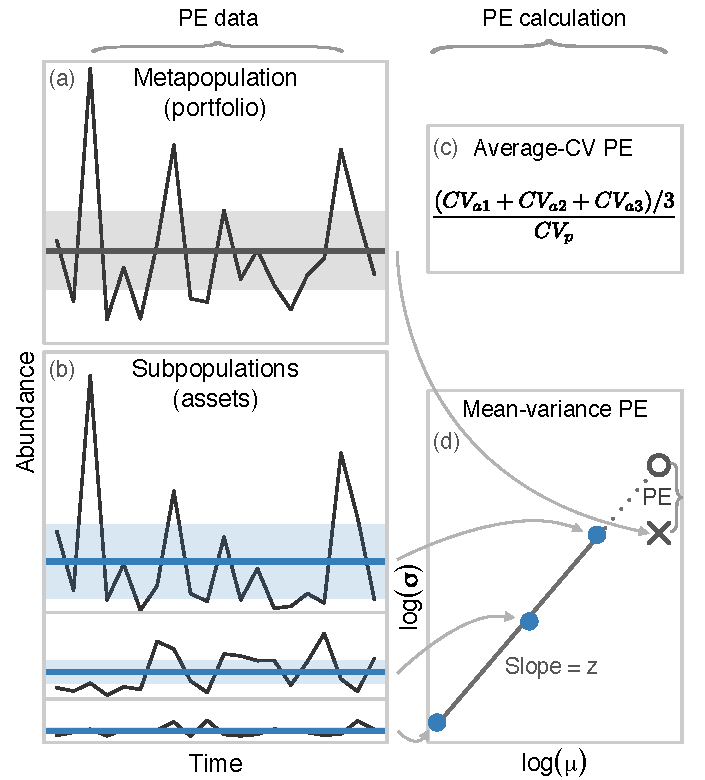
\includegraphics[height=4in]{prophets/fig1}
  \caption{
  Estimating the two PEs from empirical data. (a, b) Example
    metapopulation (portfolio) and subpopulation (asset) abundance time-series.
    Horizontal lines represent the time-series' means and the shaded regions
    represent variability. (c) We calculated the average-CV PE by dividing the
    average CV of the subpopulations ($\CV_a$) by the CV of the metapopulation
    ($\CV_p$). (d) We calculated the mean-variance PE by (1) plotting the mean
    and variance of each subpopulation on log-log axes, (2) extrapolating the
    subpopulation mean-variance relationship to the metapopulation mean
    (open-grey circle), and (3) comparing the predicted (open-grey circle) and
    observed (grey cross) metapopulation variability. Both methods will
    estimate the same PE if the slope of the log-log plot (z) equals two.
  }
  \label{fig:didactic}
\end{figure}

\clearpage
\begin{figure}[htbp]
  \centering 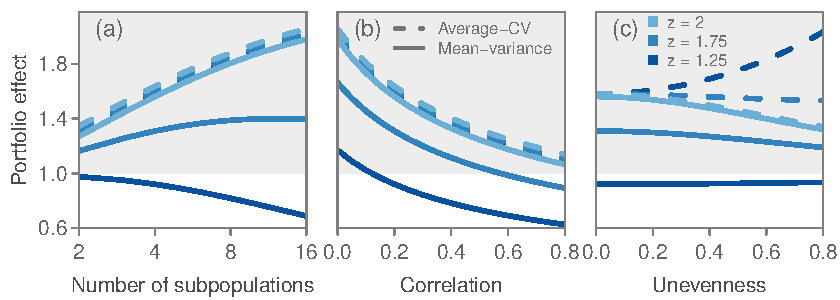
\includegraphics[width=4.8in]{prophets/fig2}
  \caption{
  The ecological factors driving the PE in theoretical systems. A PE of
    two, for example, would indicate a two-fold increase in stability for the
    portfolio compared to what we would expect in a single homogeneous
    population of the same size. We show the mean-variance PE and average-CV PE
    for three z values across (a) number of subpopulations, (b)
    correlation between subpopulation time-series, and (c) unevenness of mean
    subpopulation abundance. We generated uneven mean subpopulation abundances
    by drawing four values at quantiles of 0.2, 0.4, 0.6, and 0.8
    from a log-normal distribution
    with log-mean $\mu$ ($\mu = 2$) and log-standard deviation of the
    unevenness value (the x-axis) times $\mu$. We fixed correlation at 0.2 and subpopulation
    number at four in all panels where these parameters weren't varying. The
    grey-shading indicates stabilizing PEs. Both PE definitions are equal
    across all scenarios at z = 2. In panels (a) and (b) the average-CV PE is
    the same regardless of z.
  } \label{fig:lines}
\end{figure}

%\bigskip
\clearpage
\begin{figure}[htbp]
  \centering 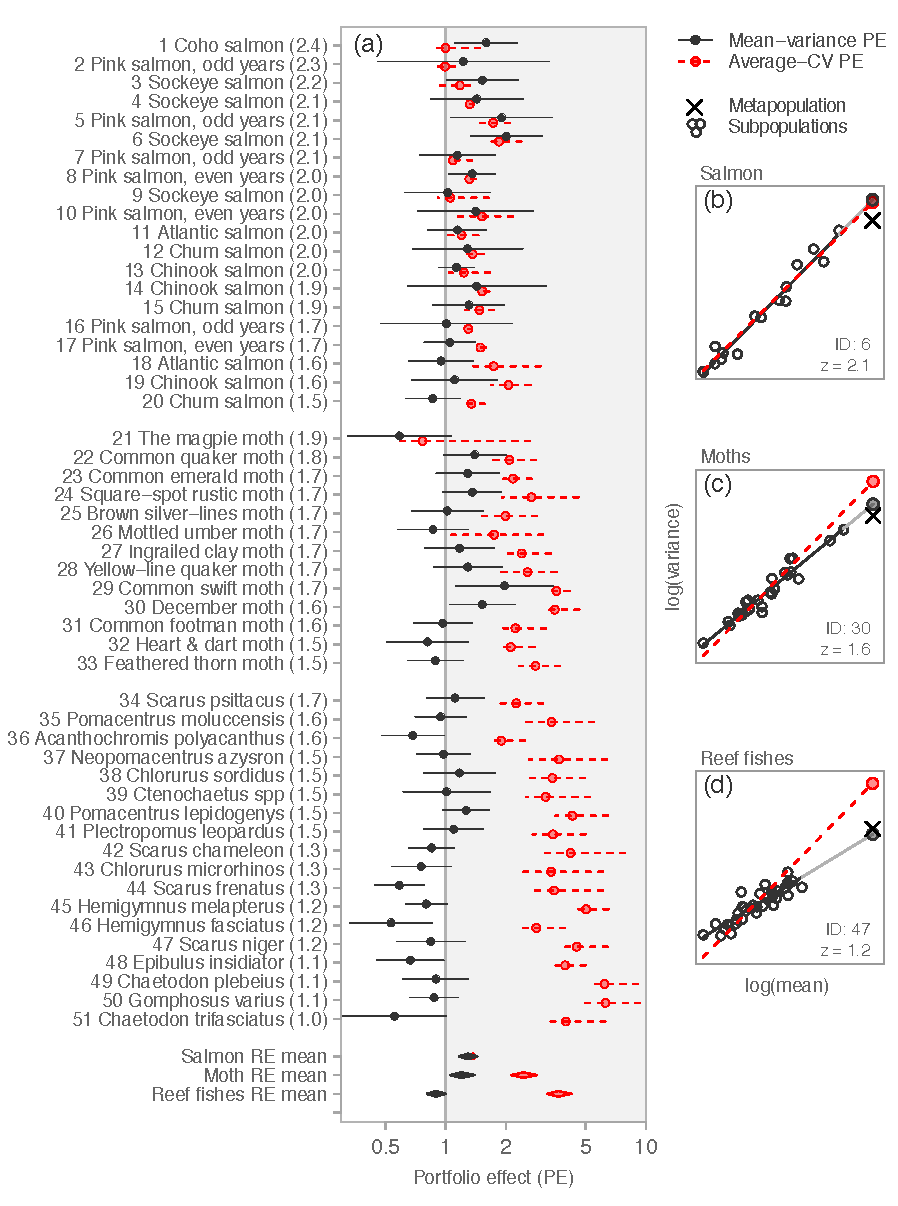
\includegraphics[height=5.5in]{prophets/fig3}
  \caption{
  PEs across 51 metapopulations. (a) Empirical PEs (circles) and 95\%
    CIs (lines) for the mean-variance method and the average-CV PE method.
    We ordered metapopulations within taxonomic groups by Taylor's law z values
    (indicated in brackets beside each metapopulation name). Diamonds represent
    inverse-variance weighted random-effect (RE) meta-analytic means and 95\%
    CIs. Numbers before population names represent population IDs (see
    Supplementary Table 1). PEs $>$ 1 (grey shading) represent stabilizing
    effects; note the log-distributed x-axis. (b, c, d) Examples of using
    Taylor's power law to calculate the mean-variance PE. The solid black
    regression line projects the subpopulation mean-variance relationship to the
    metapopulation mean abundance (shaded grey circle). The $\times$ denotes the
    observed metapopulation mean and variance. The ratio of the observed to
    predicted variance represents the mean-variance PE. The red circle denotes
    the average-CV PE and the dashed-red line the mean-variance relationship
    under the assumption that z = 2, as the average-CV PE assumes.
  }
  \label{fig:meta}
\end{figure}
%
%\bigskip
\clearpage
\begin{figure}[htbp]
  \centering 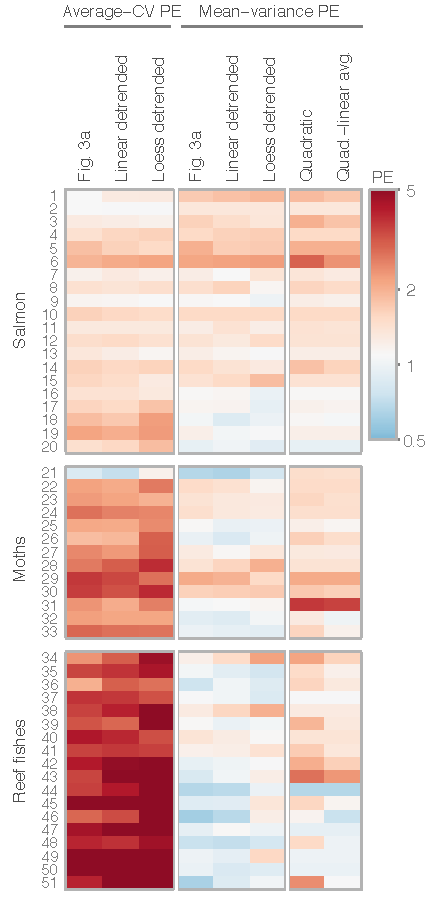
\includegraphics[height=5in]{prophets/fig4}
  \caption{
  The sensitivity of PE metrics across two detrending (linear and
    loess) methods (columns 2--3 and 5--6) and three mean-variance model fits
    (columns 4, 7--8). Columns 1 and 4 represent the same PEs as shown in
    Fig.~\ref{fig:meta}, but with colour indicating the strength of stabilizing
    effect. Red indicates a stabilizing PE, blue indicates a destabilizing PE,
    and white indicates a neutral PE. The y-axis shows the same metapopulation
    IDs as Fig.~\ref{fig:meta}.
  }
  \label{fig:detrend}
\end{figure}

%\bigskip
\clearpage
\begin{figure}[htbp]
  \centering
  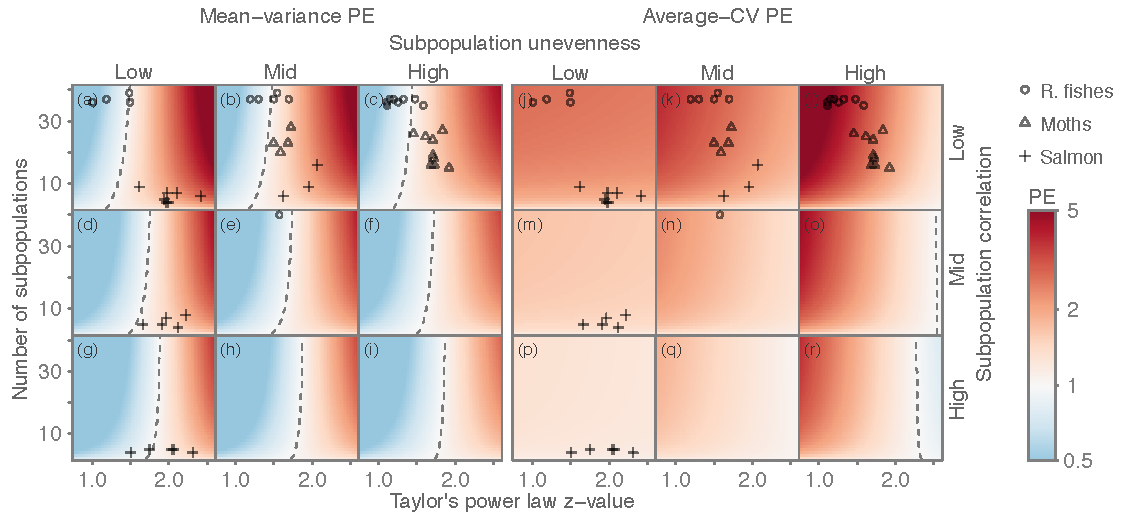
\includegraphics[width=\textwidth]{prophets/fig5}
  \caption{
  Empirical ecological PEs (points) overlaid in theoretical PE
    parameter space (colour shading). The colour shading indicates the
    stabilizing-effect of the theoretical mean-variance PEs (a--i) and
    average-CV PEs (j--r): red indicates a stabilizing effect and blue indicates
    a destabilizing effect.
    The dashed lines indicate neutral PEs. Columns from left to right
    show systems with increasingly uneven subpopulation sizes,
    and rows from top to bottom show systems with increasingly strong mean
    correlation between subpopulation (see the Supporting
    Information).
  } \label{fig:paramspace}
\end{figure}

%\bigskip
\clearpage
\begin{figure}[htbp]
  \centering 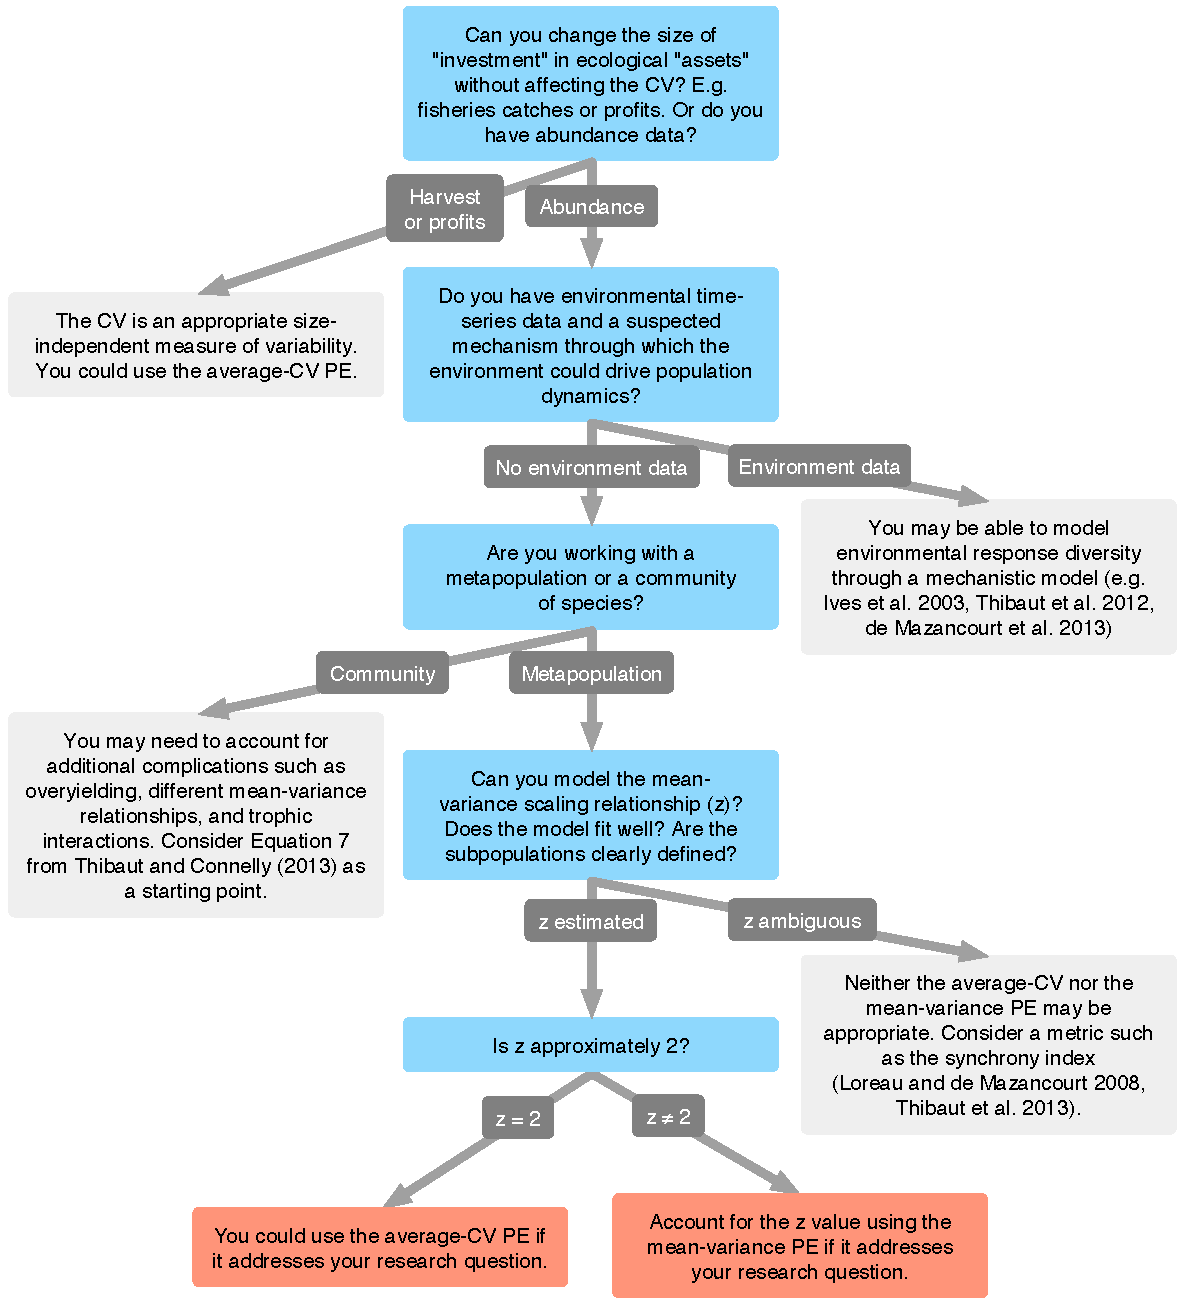
\includegraphics[width=5.2in]{prophets/fig6}
  \caption{
  %\noindent
  %\textbf{Fig.\ 6.}
  Decision tree showing options for quantifying ecological portfolios.
    Blue boxes in the middle column show questions to ask of the study system
    and available data.
    The orange boxes at the bottom represent the methods demonstrated in
    this paper. The light-grey boxes along the sides show other options to
    quantify ecological portfolios given different research questions, study
    systems, and available data.
  } \label{fig:recommendations}
\end{figure}
%
%    %\end{spacing}
%    \end{document}
